\documentclass[tikz]{standalone}
\usepackage{amsmath}
\usepackage[T1]{fontenc}
\usepackage[utf8]{inputenc}


\usetikzlibrary{arrows,%
                shapes,%
                matrix,%
                decorations.pathmorphing,%
                backgrounds,%
                positioning,%
                fit,%
                petri}

%\usetikzlibrary{external}
%\tikzexternalize[prefix=tikz/]
\usepackage{mathpazo}

\begin{document}

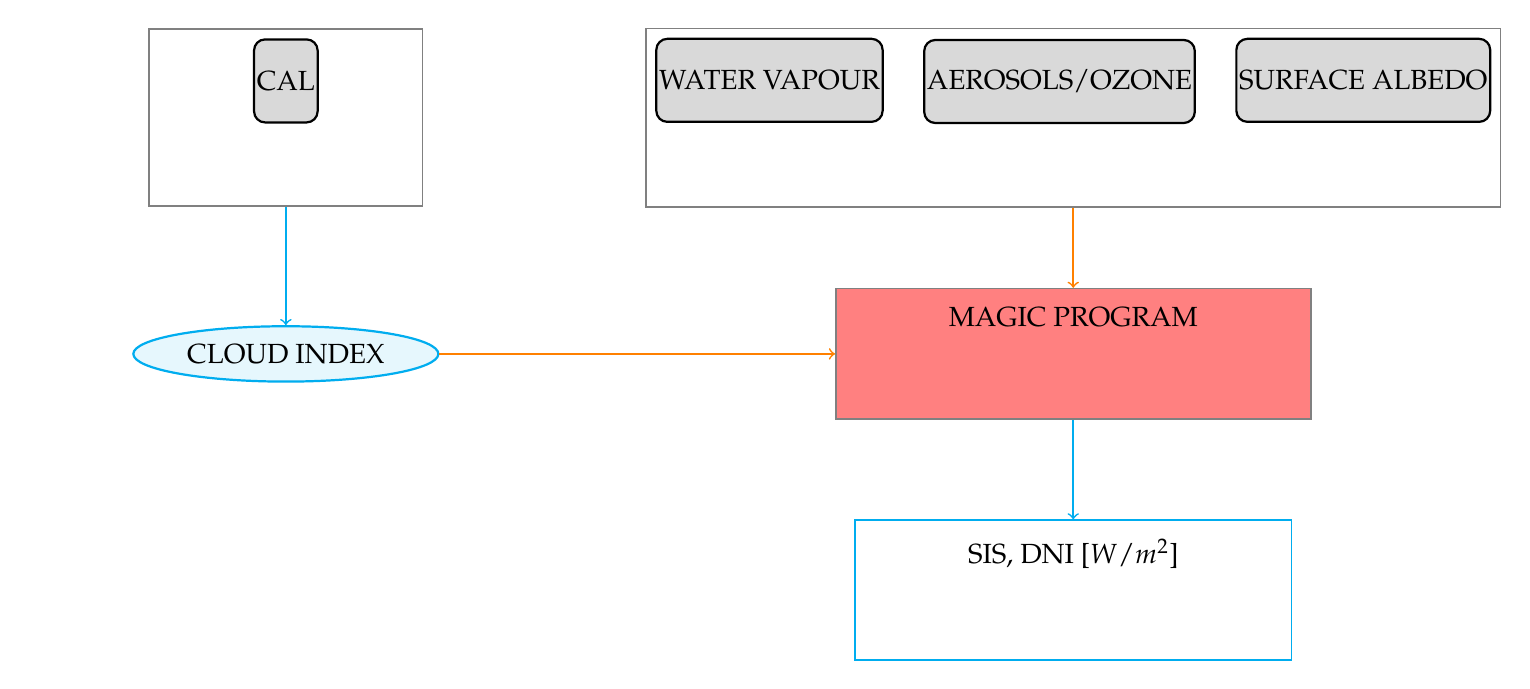
\begin{tikzpicture}[auto,
operation/.style={rectangle, rounded corners, draw=black, thick, fill=gray!30,
minimum height=3em, align=flush center, inner sep=1pt},
%
simple/.style={draw=black, circle, fill=gray!30},
%
source/.style ={draw=orange, thick, ellipse, fill=orange!10,
minimum height=2em},
%
result/.style ={draw=cyan, thick, ellipse, fill=cyan!10,
  minimum height=2em},
%
method/.style={draw=yellow, thick, ellipse, fill=yellow!10,
minimum height=2em}]

\tikzset{every path/.style={line width=.6pt}}

% \begin{scope}[xshift=+9cm]
%   \matrix[matrix of nodes, fill=white, draw=white, column sep=5mm, row sep=7mm, minimum width=7mm] (Solar Data){
%         \node  {}; &
%         \node  {}; &
%         \node  {}; \\
%         %%%%%%%%%%%%%%%%%%%%%%%%%%%%%%%%%%
%         \node {}; &
%         \node [source] (GHI) {Solar Irradiation}; &
%         \node {}; \\
% };
% \end{scope}

\begin{scope}[yshift=-1cm]
  \matrix[matrix of nodes, fill=white, draw=black!50, column sep=5mm, row sep=7mm, minimum width=7mm] (OBS){
        \node  {}; &
        \node  [operation] (cal) {CAL}; &
        \node  {}; \\
        %%%%%%%%%%%%%%%%%%%%%%%%%%%%%%%%%%
        \node {}; &
        \node {}; &
        \node {}; \\
};
\end{scope}

\begin{scope}[yshift=-1cm, xshift=10cm]
  \matrix[matrix of nodes, fill=white, draw=black!50, column sep=5mm, row sep=7mm, minimum width=7mm] (CLIMATOLOGY){
        \node  [operation] (vapour){WATER VAPOUR}; &
        \node  [operation] (aero) {AEROSOLS/OZONE}; &
        \node  [operation] (albedo) {SURFACE ALBEDO}; \\
        %%%%%%%%%%%%%%%%%%%%%%%%%%%%%%%%%%
        \node {}; &
        \node {}; &
        \node {}; \\
};
\end{scope}

\begin{scope}[yshift=-4cm, xshift=10cm]
  \matrix[matrix of nodes, fill=red!50, draw=black!50, column sep=5mm, row sep=7mm, minimum width=7mm] (MAGIC){
        \node  {}; &
        \node  (Magic) {MAGIC PROGRAM}; &
        \node  {}; \\
        %%%%%%%%%%%%%%%%%%%%%%%%%%%%%%%%%%
        \node {}; &
        \node {}; &
        \node {}; \\
};
\end{scope}

\begin{scope}[yshift=-7cm, xshift=10cm]
  \matrix[matrix of nodes, fill=white, draw=cyan, column sep=5mm, row sep=7mm, minimum width=7mm] (RESULTS){
        \node  {}; &
        \node  (Results) {SIS, DNI [$W/m^2$]}; &
        \node  {}; \\
        %%%%%%%%%%%%%%%%%%%%%%%%%%%%%%%%%%
        \node {}; &
        \node {}; &
        \node {}; \\
};
\end{scope}

% \begin{scope}[yshift=-5cm, xshift=10cm]
%   \matrix[matrix of nodes, fill=white, draw=white, column sep=5mm, row sep=6mm, minimum width=7mm] (Prod results){
%         \node  {}; &
%         \node  [result] (Fixed) {Fixed}; &
%         \node  {}; \\
%         %%%%%%%%%%%%%%%%%%%%%%%%%%%%%%%%%%
%         \node {}; &
%         \node [result] (Horiz) {1axis}; &
%         \node {}; \\
%         %%%%%%%%%%%%%%%%%%%%%%%%%%%%%%%%%%
%         \node {}; &
%         \node [result] (Two) {2axes}; &
%         \node {}; \\
% };
% \end{scope}
 
% \begin{scope}[yshift=-5cm, xshift=15cm]
%   \matrix[matrix of nodes, fill=gray!10, draw=black!50, column sep=5mm, row sep=7mm, minimum width=7mm] (Variabilidad){
%         \node  {}; &
%         \node  [operation] (Variability) {Variability}; &
%         \node  {}; \\
%         %%%%%%%%%%%%%%%%%%%%%%%%%%%%%%%%%%
%         \node {}; &
%         \node {}; &
%         \node {}; \\
% };
% \end{scope}

% \begin{scope}[yshift=-5cm, xshift=20cm]
%   \matrix[matrix of nodes, fill=white, draw=white, column sep=5mm, row sep=5mm, minimum width=7mm] (Variability results){
%         \node  {}; &
%         \node  [result] (CVirradiation) {$CV_{GHI}$}; &
%         \node  {}; \\
%         %%%%%%%%%%%%%%%%%%%%%%%%%%%%%%%%%%
%         \node {}; &
%         \node [result] (CVfixed) {$CV_{fixed}$}; &
%         \node {}; \\
%         %%%%%%%%%%%%%%%%%%%%%%%%%%%%%%%%%%
%         \node {}; &
%         \node [result] (CVHoriz) {$CV_{1axis}$}; &
%         \node {}; \\
%         %%%%%%%%%%%%%%%%%%%%%%%%%%%%%%%%%
%         \node {}; &
%         \node [result] (CVTwo) {$CV_{2axes}$}; &
%         \node {};\\
% };
% \end{scope}


\begin{scope}[yshift=-4cm]
  \matrix[matrix of nodes, fill=white, draw=white, column sep=5mm, row sep=7mm, minimum width=7mm] (cloud){
        \node  {}; &
        \node  [result] (cloudindex) {CLOUD INDEX}; &
        \node  {}; \\
};
\end{scope}

% \begin{scope}[yshift=-8cm, xshift=10cm]
%   \matrix[matrix of nodes, fill=gray!10, draw=black!50, column sep=5mm, row sep=7mm, minimum width=7mm] (by cluster){
%         \node  {}; &
%         \node  [operation] (mask apply) {aggregating by cluster}; &
%         \node  {}; \\
% };
% \end{scope}

% \begin{scope}[yshift=-10cm, xshift=10cm]
%   \matrix[matrix of nodes, fill=white, draw=white, column sep=5mm, row sep=7mm, minimum width=7mm] (after mask){
%         \node  {}; &
%         \node  [result] (after mask result) {Results by cluster}; &
%         \node  {}; \\
% };
% \end{scope}

% \begin{scope}[yshift=-12cm, xshift=10cm]
%   \matrix[matrix of nodes, fill=gray!10, draw=black!50, column sep=5mm, row sep=7mm, minimum width=7mm] (Complementarity){
%         \node  {}; &
%         \node  [operation] (complementariedad) {Complementarity}; &
%         \node  {}; \\
% };
% \end{scope}

% \begin{scope}[yshift=-12cm, xshift=17cm]
%   \matrix[matrix of nodes, fill=white, draw=white, column sep=5mm, row sep=7mm, minimum width=7mm] (Complemtarity results){
%         \node  {}; &
%         \node  [result] (complementarity results) {Complementarity results}; &
%         \node  {}; \\
% };
% \end{scope}


\begin{scope}
  \draw[->, orange](cloudindex.east) -- (MAGIC.west);
  \draw[->, orange](CLIMATOLOGY.south) -- (MAGIC.north);
  %%%%%%%%%%%%%%%%%%%%%%%%%%%%%%%%%%%%%
  \draw[->, cyan](OBS.south) -- (cloudindex.north);
  %%%%%%%%%%%%%%%%%%%%%%%%%%%%%%%%%%%%
  \draw[->, cyan](MAGIC.south) -- (RESULTS.north);
\end{scope}


\end{tikzpicture}

\end{document}
